\documentclass[12pt,a4paper]{article}

% --- Kodowanie i język ---
\usepackage[utf8]{inputenc}
\usepackage[T1]{fontenc}
\usepackage[polish]{babel}

% --- Marginesy A4 ---
\usepackage[a4paper,margin=2.5cm]{geometry}

% --- Grafika ---
\usepackage{graphicx}

% --- Matematyka ---
\usepackage{amsmath, amssymb}

% --- Linki ---
\usepackage{hyperref}

% --- Wcięcia i odstępy ---
\usepackage{parskip}

% --- Nagłówek i stopka ---
\usepackage{fancyhdr}
\pagestyle{fancy}
\fancyhf{}
\lhead{Opis kodu Morse’a}
\rhead{\leftmark}
\cfoot{\thepage}

% --- Tytuł ---
\title{Opis kodu Morse’a}
\author{SP5YAM}
\date{\today}

\begin{document}

\maketitle
\newpage
\tableofcontents
\newpage

% --- Sekcje ---
\section{Prędkość nadawania}


Prędkość nadawania morsem liczymy w tzw. WPM (words per minute).

Prędkość w WPM mówi nam ile razy jesteśmy w stanie wysłać słowo PARIS w ciągu jednej minuty.

Przykładowo 10 WPM oznacza że jesteśmy w stanie nadać 10 słów PARIS w ciągu jednej minuty.

\subsection{Czas trwania symboli}


Podstawową jednostką czasu kodu morsa jest czas nadawania kropki.
Tabela przedstawia czas trwania poszczególnych elementów:

\begin{tabular}{|c|c|}
	\hline
	Opis elementu & Czas trwania \\
	\hline
	Symbol - Kropka	& 1 kropka – jednostka podstawowa \\
	\hline
	Symbol - Kreska & 3 kropki \\
	\hline
	Odstęp między symbolami & 3 kropki \\
	\hline
	Odstęp między wyrazami & 7 kropek \\
	\hline
	Słowo "PARIS " ze spacją na końcu & 50 kropek  \\
	\hline
\end{tabular}


\subsection{Ile czasu trwa kropka?}


Podstawową jednostką kodu morsa jest kropka. Aby obliczyć jej czas trwania musimy przeliczyć to z jednostki WPM.

Słowo PARIS wraz z przerwą zajmuje 50 kropek:

\begin{figure}[h]
	\centering
	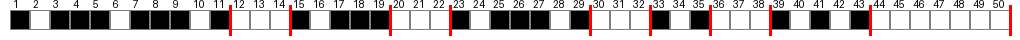
\includegraphics[width=0.95\textwidth]{images/morse_timeline.png}
	\caption{Wykres kodu Morse’a dla sekwencji PARIS + spacja}
	\label{fig:morse}
\end{figure}

Czas trwania jednej kropki (w sekundach) liczymy zatem ze wzoru:

\begin{equation}
	T_{\text{kropka}} = \frac{60}{50 \cdot \text{WPM}}
\end{equation}

Czas trwania kropki dla różnych WPM można przedstawić dla zobrazowania w tabeli:

\begin{tabular}{|c|c|}
	\hline
	WPM & Czas kropki (s) \\
	\hline
	5 & 0.2400 \\
	\hline
	6 & 0.2000 \\
	\hline
	7 & 0.1714 \\
	\hline
	8 & 0.1500 \\
	\hline
	9 & 0.1333 \\
	\hline
	10 & 0.1200 \\
	\hline
	11 & 0.1091 \\
	\hline
	12 & 0.1000 \\
	\hline
	13 & 0.0923 \\
	\hline
	14 & 0.0857 \\
	\hline
	15 & 0.0800 \\
	\hline
	16 & 0.0750 \\
	\hline
	17 & 0.0706 \\
	\hline
	18 & 0.0667 \\
	\hline
	19 & 0.0632 \\
	\hline
	20 & 0.0600 \\
	\hline
	21 & 0.0571 \\
	\hline
	22 & 0.0545 \\
	\hline
	23 & 0.0522 \\
	\hline
	24 & 0.0500 \\
	\hline
	25 & 0.0480 \\
	\hline
	26 & 0.0462 \\
	\hline
	27 & 0.0444 \\
	\hline
	28 & 0.0429 \\
	\hline
	29 & 0.0414 \\
	\hline
	30 & 0.0400 \\
	\hline
	31 & 0.0387 \\
	\hline
	32 & 0.0375 \\
	\hline
	33 & 0.0364 \\
	\hline
	34 & 0.0353 \\
	\hline
	35 & 0.0343 \\
	\hline
	\hline
\end{tabular}





\end{document}
